 %\documentclass[wcp,gray]{jmlr} % test grayscale version
\documentclass[wcp]{jmlr}

 % The following packages will be automatically loaded:
 % amsmath, amssymb, natbib, graphicx, url, algorithm2e

 %\usepackage{rotating}% for sideways figures and tables
\usepackage{longtable}% for long tables
\usepackage{booktabs}
\usepackage{tikz}
\usetikzlibrary{arrows,positioning} 
% \usepackage[load-configurations=version-1]{siunitx} % newer version
 %\usepackage{siunitx}
 
 \tikzset{
    %Define standard arrow tip
    >=stealth',
    %Define style for boxes
    observed/.style={
           circle,
           rounded corners,
           draw=black, thick,
           minimum width=2.2em,
           minimum height=2.2em,
           font=\footnotesize,
           text centered,
           },
     latent/.style={
           circle,
           rounded corners,
           draw=black, thick, dashed,
           minimum width=2.2em,
           minimum height=2.2em,
           font=\footnotesize,
           text centered,
           fill=black!10!white
           },
    target/.style={
           circle,
           rounded corners,
           draw=black, thick,
           minimum width=2.2em,
           minimum height=2.2em,
           font=\footnotesize,
           text centered,
           fill=black!20!white,
           },
    observedrect/.style={
           rectangle,
           rounded corners,
           draw=black, thick,
           minimum width=6em,
           minimum height=2em,
           font=\footnotesize,
           text centered,
           },
     targetrect/.style={
           rectangle,
           rounded corners,
           draw=black, thick,
           minimum width=6em,
           minimum height=2em,
           font=\footnotesize,
           text centered,
           fill=black!20!white,
           },
     empty/.style={
           circle,
           rounded corners,
           minimum width=.5em,
           minimum height=.5em,
           font=\footnotesize,
           text centered,
           },
    % Define arrow style
    pil/.style={
           o->,
           thick,
           shorten <=2pt,
           shorten >=2pt,},
    sh/.style={ shade, shading=axis, left color=red, right color=green,
    shading angle=45 }   
}

% change the arguments, as appropriate, in the following:
\jmlrvolume{NNN}
\jmlryear{2015}
\jmlrworkshop{ICML}

\title[Causal Bandits]{Causal Bandits}

 % Use \Name{Author Name} to specify the name.
 % If the surname contains spaces, enclose the surname
 % in braces, e.g. \Name{John {Smith Jones}} similarly
 % if the name has a "von" part, e.g \Name{Jane {de Winter}}.
 % If the first letter in the forenames is a diacritic
 % enclose the diacritic in braces, e.g. \Name{{\'E}louise Smith}

 % Authors with different addresses:
 % \author{\Name{Author Name1} \Email{abc@sample.com}\\
 % \addr Address 1
 % \AND
 % \Name{Author Name2} \Email{xyz@sample.com}\\
 % \addr Address 2
 %}
\author{\Name{Author's Name}}

\editor{Editor's name}
 % \editors{List of editors' names}

\begin{document}

\maketitle

\begin{abstract}
	The abstract
\end{abstract}
\begin{keywords}
	Causality, Bandits, Regret Bounds
\end{keywords}

\section{Introduction}
\label{sec:intro}

The aim of this paper is to demonstrate theoretically the utility of having 
causal knowledge when solving multi-armed bandit (MAB) problems.

We do this by:
\begin{enumerate}
	\item Providing some motivating examples as to why it is reasonable to expect to have some knowledge of causal structures when solving a sequential decision making problem such as MAB problems.
	\item Formalising what we mean by ``causal information'' for a simple 	class of stochastic multi-armed bandit (MAB) problems. 
	
	We can formalize a connection between causal graphs and fairly general stochastic MAB problems (section 4 of my TPR)
	
	\item Demonstrating that knowledge of causal structure can induce interesting dependencies between the rewards of different MAB arms.
	
	Described in section 4 of my TPR
	
	\item Introducing a specific causal MAB problem demonstrating this structure and proposing a simple explore-then-exploit algorithm that makes use of the causal information and yields significant improvements over the corresponding lower bounds for algorithms that do not use the causal information.

Given the causal structure in figure \ref{fig:causalStructure} we get an upper bound $R(T) = m^{1/3}T^{2/3}log(KT)^{1/3}$ (section 1 of observe-then-best, section 1.1 if $\boldsymbol{q}$ is not known in advance).  Where $m$ can be interpreted as the number of arms corresponding to variable settings that occur only rarely if not explicitly set. The corresponding lower bound for algorithms that do not leverage causal structure is  $\sqrt{KT}$ (Auer1995). This demonstrates the causal algorithm will do significantly better where there are large number of arms, provided $m$ is not too large.
\begin{figure}[H]
\centering
\caption{Assumed Causal Structure}
\label{fig:causalStructure}
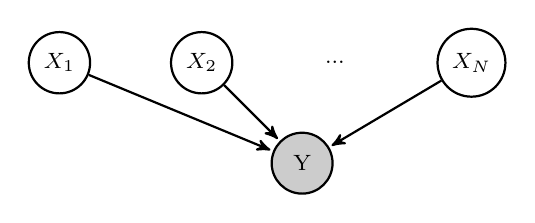
\begin{tikzpicture}[->,>=stealth',shorten >=1pt,auto,node distance=1cm,
  thick,main node/.style={observed}, hidden/.style={empty},tg/.style={target}]

 %nodes
\node[main node](1){$X_{1}$};
\node[main node, right=of 1](2){$X_{2}$};
\node[hidden, right=of 2](3){$...$};
\node[main node, right=of 3](4){$X_{N}$};
\node[tg, below right=of 2](5){Y};
 \path[every node/.style={font=\sffamily\small}]
    (1) edge (5)
    	(2) edge (5)
    (4) edge (5);
	
\end{tikzpicture}
\end{figure}
	
	\item Deriving a matching lower bound for this problem for algorithms that make use of the causal structure.
	
	We currently have (lowerbounds-auer section 3) a lower bound of $m^{1/3}T^{2/3}$ for algorithms that use information provided by purely observing. Ie the structure introduced by equation 6 in my TPR. This bound does not apply to algorithms using information in the form provided by equation 7 in my TPR. (ie we have not yet shown that we are fully utilizing the causal information available).
	
	\item Demonstrating we can also use the causal structure to gain significant improvement for the closely related best-arm identification problem.
	
	We obtain simple regret $R_s(T) = \sqrt{m/T}$ (observe-then-best section 1.1) versus $R_s(T) = \sqrt{K/T}$ for the non-causal version of the problem (Bubeck et al 2009)
	
	
\end{enumerate}

We identify a problem-dependent constant that appears in the upper and lower 
bounds that can be roughly interpreted as a measure of how much actions reveal
about other actions via the causal structure.

\subsection{Related Work}
\label{sub:related_work}

\begin{itemize}
	\item Bareinboim, Forney \& Pearl, \emph{Bandits with unobserved 
			confounders}, NIPS 2015
	\item Salomon, Audibert \& Alaoui, \emph{Lower Bounds and Selectivity of 
			Weak-Consistent Policies in Stochastic Multi-Armed Bandit Problems},
			JMLR 2013.
	\item Alon, Cesa-Bianchi, Dekel, Koren, \emph{Online Learning with Feedback
			Graphs: Beyond Bandits}, COLT 2015.
\end{itemize}


% \acks{Acknowledgements go here.}

\bibliography{all.bib}

\end{document}
